\documentclass[12pt, twoside]{article}
\usepackage[letterpaper, margin=1in, headsep=0.5in]{geometry}
\usepackage[english]{babel}
\usepackage[utf8]{inputenc}
\usepackage{amsmath}
\usepackage{amsfonts}
\usepackage{amssymb}
\usepackage{tikz}
\usetikzlibrary{quotes, angles}
\usepackage{venndiagram}
\usepackage{multicol}

\usepackage{fancyhdr}
\pagestyle{fancy}
\fancyhf{}
\renewcommand{\headrulewidth}{0pt} % disable the underline of the header

\fancyhead[RE]{\thepage}
\fancyhead[RO]{\thepage \\ Name: \hspace{3cm}}
\fancyhead[L]{BECA / Dr. Huson / IB Math\\* 27 September 2019}


\begin{document}
\subsubsection*{1.16 Exit Note Quiz: Trigonometry skills}

\begin{enumerate}

  \item Solve the given triangle (determine the values of all lengths and angles)
  \begin{center}
    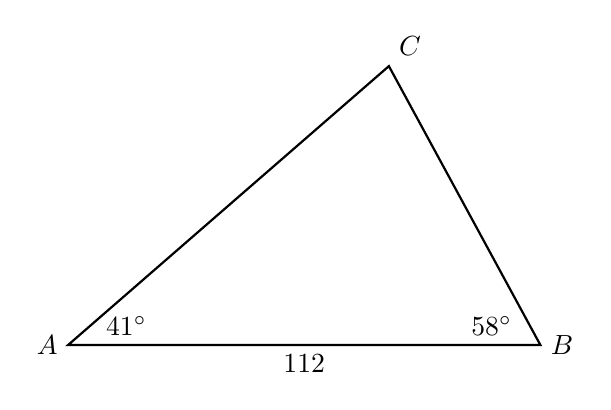
\begin{tikzpicture}[scale=1.2]
      \draw [-, thick] (41:4.5) node[above right]{$C$}--
        (0,0) node[left]{$A$}--
        (5,0) node[right]{$B$}--cycle;
      \node at (0.3, 0)[above right]{$41^\circ$};
      \node at (4.8, 0)[above left]{$58^\circ$};
      \node at (2.5, 0)[below]{$112$};
    \end{tikzpicture}
    \end{center} \vspace{1cm}

    \item Find the slant height of a cone with a diameter of 32 centimeters and height of 12 cm. \vspace{1cm}
    
    \item Triangle $ABC$ has an area of 100, with $AB=15$ and $AC=17$. Find the measure of the angle $A$. \\[0.5cm]
    Hint: Consider that the two configurations shown have the same base and altitude.
    \begin{flushleft}
      \begin{tikzpicture}[scale=0.3]
        \draw [-, thick] (51.7:17) node[above right]{$C$}--
          (0,0) node[left]{$A$}--
          (15,0) node[right]{$B$}--cycle;
        \node at (1, 0)[above right]{$\theta$};
        \node at (5, 7)[above left]{$17$};
        \node at (8, 0)[below]{$15$};

      \begin{scope}[shift={(35,0)}]
          \draw [-, thick] ({180-51.7}:17) node[above right]{$C'$}--
            (0,0) node[left]{$A'$}--
            (15,0) node[right]{$B'$}--cycle;
          \node at (0, 0)[above right]{$180-\theta$};
          \node at (-5.5, 5)[above left]{$17$};
          \node at (8, 0)[below]{$15$};
      \end{scope}

      \draw [-, dashed] (11.5,13.33)--(24,13.33);

      \end{tikzpicture}
      \end{flushleft} 


\end{enumerate}
\end{document}
